\chapter{Testing and Evaluation}



\section{Introduction}

In order to answer our research questions of how to improve the performance of
Web services in DIL environments, we developed test setups and environments to
evaluate the proxy. The goal is to measure any possible improvements(or
deterioration) of performance when we use the proxy developed as a part of this
thesis. In this chapter we present how the testing was performed and finally
present the results we obtained. Since the proxy is being developed as a
prototype for military usage, we wanted to use test scenarios that resembles
actual military and civilian usage.  While W3C services only uses HTTP as a
transport mechanism, REST utilizes the different HTTP methods to indicate which
operation to perform on a resource. Each test scenario is therefor performed
with both a W3C Web service applications and RESTful Web services.

To evaluate how different network properties affects performance, the tests
was performed on networks with different characteristics. The base case was to
test without any intentional limitations to the network and without the actual
usage of the proxy. Then we introduced usage of the proxy and evaluated it in
different types of networks. An infinite number of possible network
combinations exists, so we have in this thesis chosen to focus on five
different network types identified by the task group IST-118 for DIL-testing.
The different networks are summarized in \cref{table-network-types}.

Furthermore we performed tests with two setups, first with machine-to-machine
over an Ethernet cable, then over actual military communication equipment. The
usage of actual military equipment allowed us to get as realistic results as
possible.


\section{Evaluation Tools}

In order to simulate \gls{dil} environments we need some way to control the
properties of the network traffic. In this thesis we use two approaches, the
first one connecting two machines through a third machine. The third machine
will use a component of the linux kernel to control the flow of the network
traffic flowing through it, allowing us to simulate a DIL network. The second
approach involves using actual military equipment in laboratory at FFI. The
benefit of using actual equipment, is that we get as realistic tests as
possible.

\subsection{\glsentrylong{netem}}

Fortunately, the Linux kernel offers a rich set of tools for managing and
manipulating the transmission of packets. \gls{netem} is an enchancement of the
traffic control facilities that allows us to control delay, packet loss and
other characteristics to packets outgoing from a selected network interface.
\Cref{figure-testing-environment} illustrates the setup of this approach.

%Siter man-page om tc-netem
%Siter tldp -> Traffic Control HOWTO



\textbf{tc}(traffic control) is a linux program to configure and control the
linux kernels Network scheduler. This program allows us to emulate many of the
network characteristics that DIL has and the different setups are explained in
the coming sections.

\subsubsection{Delays}

NetEm can emulate delays on packets on a specific link.

\begin{lstlisting}[frame=single, caption="Emulating delay"]
  tc qdisc add dev eth0 root netem delay 100ms
\end{lstlisting}

In this example we add a fixed delay on 100 ms to all packets going out of local
Ethernet.


\section{Test Setup}
\label{testing-environment}

The majority of testing was performed on machines located at the FFI-lab at
Kjeller. Although testing on regular machines gives us a indication, to get as
realistic results as possible we also performed tests on military communication
equipment.

The Web service and client are connected to each other through a third
computer, acting as a router. This router machine had two network cards and
networked together the other machines by Ethernet cables. In order for the
router machine to forward IP packets back and forth between the client and
server, IP forwarding was enabled on the kernel. The specifications of the
machines involded in the testing are listed in \cref{table-machines}.

\begin{figure}[h]
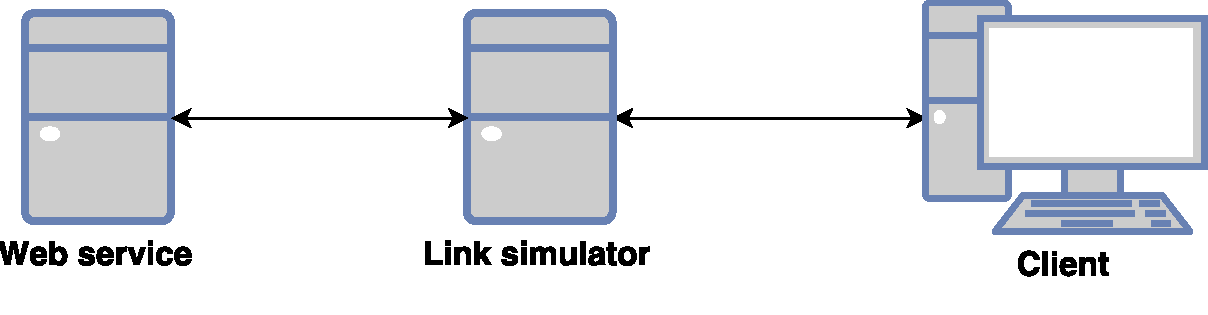
\includegraphics[scale=0.6]{images/testing_environment.pdf}
\caption{Testing environment}
\label{figure-testing-environment}
\end{figure}


\begin{table}[h]
\begin{tabular}{| l | l | l |}
\hline
  \textbf{Role} & \textbf{OS} & \textbf{Kernel version}\\ \hline
  Client & Debian & 2.16 \\ \hline
  Web service & Ubuntu & 2.15 \\ \hline
  Router & Ubuntu & 2.15 \\ \hline
\end{tabular}
\caption{Machines involved in the testing}
\label{table-machines}
\end{table}


The server and client are assigned an IP address in two different subnets.
This is done by the Linux network interface administration program
\textit{ifconfig}. In \cref{listing-ifconfig-client} the client machine is is
assigned the IP address 192.168.2.44.

\begin{lstlisting}[frame=single, caption="Configuring a network interface of the router", label=listing-ifconfig-client]
ifconfig eth0 192.168.2.1 up
\end{lstlisting}

After setting up the IP addresses we need to configure the routing so that the
kernel know where to route the network traffic. In this case we want all
traffic to go through the routing machine. In \cref{listing-routing} we
configure all IP traffic boud for the subnet 192.168.1.X to be routed through
the router machine with IP 192.168.2.1.

\begin{lstlisting}[frame=single, caption="Configuring routing rules for the client", label=listing-routing]
ip route add unicast 192.168.1.0/24 via 192.168.2.1
\end{lstlisting}


\subsection{Enabling proxies}

In order to enable the applications to tunnel all their HTTP traffic through our
proxy, we needed a way to setup a proxy without altering the applications
themselves. Fortunately, Java provide mechanisms to deal with
proxies\cite{oracle-proxy}. We configured the \gls{jvm} to get the applications
to tunnel all HTTP traffic through our proxy. This is done by setting properties
to the \gls{jvm}:


\begin{lstlisting}[frame=single, caption="Setting a proxy on the \gls{jvm}", label=test]
java -Dhttp.proxyHost=localhost \
-Dhttp.proxyPort=3001 \
-Dhttp.nonProxyHosts= \
-jar target/client.jar
\end{lstlisting}

In \cref{test} the application \textbf{client.jar} is started and all HTTP
traffic will go through the proxy server at localhost on port 3001.

\subsection{Emulating networks}

Since all network traffic passes through the routing machine, we can control
the flow of IP packets here. As previously discussed, we use Netem.  For each
network configuration, a bash script is run. This script configures the
network interfaces in order to get the correct network behaviour. Both
interfaces are configured so the network is symmetrical in both directions.

\section{Test Execution}

In our tests we use two different sets of applications. One for W3C Web services
and one for RESTful  Web services. Data being sent between the client and server
is sent uncompressed.

\subsection{W3C Web service test applications}

For the purpose of testing W3C Web service applications we simulated a system
which allows units in the field to report positions of friendly forces back to
a headquarter. The position reports use the \gls{nffi} format, which has an
associated XML schema with it.

The client requests these data over the network. This is repeated x times and
the the average round-trip time is calculated. The test service was deployed
with Glassfish 4, an application server. The client was ran through the IDEA
Netbeans.


\subsection{RESTful Web service test applicatons}

For testing we developed a small RESTful Web service, an example service
keeping order of cars in a ``car system''. The service exposes an \gls{api}
which offers different operations to manage the car system. Clients can invoke
these operations by using HTTP requests and utilizing the associated HTTP
method to indicate what to do with an resource. Since RESTful services are
payload agnostic, we choose JSON to represent the data being sent between the
server and the client. JSON is a lightweight data-format.

Each test case consist of a client sequentially invoking the server with
different API requests. The most common HTTP-methods GET, PUT, POST, and
DELETE are all part of the testing.



\subsection{Test parameters}

\begin{itemize}
	\item Compression on/off.
	\item Proxy on/off.
    \item Transport protocol
    \item Message size
\end{itemize}

\subsection{Testing on military communication equipment}

To verify the results from the other tests, we also wanted to run some of the
tests as close to reality as possible. We therefore used Kongsberg radios.

\section{Function tests}

The first phase of the testing was performed without any actual intended
limitations to the network. The objective of this testing is to validate that
the proxy is working correctly and have a benchmark to compare other results
with. This phase was again divided into two phases, one without the usage of
proxy and one with the usage of it. This allows us to investigate any potential
overhead associated with the usage of the proxy.

\subsection{Execution}

The Web service client and the service itself was started on separately machines
interconnected through a third machines acting as a router as discussed in
\cref{testing-environment}. However for the first phase, the client and server
did not use any proxy.

Warm-up.

Number of tests.

Delay less than 1 ms.
Iperf bandwidth: 7.76 Mbits/sec


\subsection{Results and Analysis}

Enabling compression yields an improvement in the performance. We also notice
that HTTP and CoAP has a almost identical performance, while AMQP has
significant longer RTT.

\begin{table}[h!]
\begin{tabular}{| l | l | l |}
\hline
  \textbf{Test} & \textbf{Avg. RTT} & \textbf{With compression}\\ \hline
  Without proxy & 122 ms & N/A \\ \hline
  Proxy with HTTP & 163 ms & 99 ms \\ \hline
  Proxy with AMQP & 529 ms & 490 ms \\ \hline
  Proxy with CoAP & 284 ms & 122 ms \\ \hline
\end{tabular}
\caption{W3C Web service results}
\end{table}

\begin{table}[h!]
\begin{tabular}{| l | l | l |}
\hline
  \textbf{Test} & \textbf{Transfer time} & \textbf{With compression}\\ \hline
  Without proxy & 244 ms & N/A \\ \hline
  Proxy with HTTP & 368 ms & 337\\ \hline
  Proxy with AMQP & 2084 ms & 2040\\ \hline
  Proxy with CoAP & 331 ms & 334\\ \hline
\end{tabular}
\caption{RESTful Web service results}
\end{table}


\section{DIL Tests - Disconnected}

In this scenario we evaluate  the performance with the DIL characteristic
\textit{disconnected}, which refers to the network suddenly going down when the
application is sending data. The objective of this testing is to evaluate how
the proxy manages disconnects over longer periods of time. We define the success
criteria for this test to be that the client is able to eventually process his
request after the connection is reestablished. The client HTTP request should
not be interrupted in any way, other than it taking longer time to process the
request.

\subsection{Execution}

 The tests are performed on a unlimited network. During testing we physically
 remove the Ethernet cable during transmission. 60 seconds?

\subsection{Results}

\begin{table}[h!]
\begin{tabular}{| l | l |}
\hline
  \textbf{Test} & \textbf{Result} \\ \hline
  Without proxy & Timeout \\ \hline
  Proxy with HTTP & Success \\ \hline
  Proxy with AMQP & Success \\ \hline
  Proxy with CoAP & Success \\ \hline
\end{tabular}
\caption{W3C Web service results}
\end{table}

\begin{table}[h!]
\begin{tabular}{| l | l |}
\hline
  \textbf{Test} & \textbf{Result} \\ \hline
  Without proxy & Timeout \\ \hline
  Proxy with HTTP & Success \\ \hline
  Proxy with AMQP & Success \\ \hline
  Proxy with CoAP & Success \\ \hline
\end{tabular}
\caption{RESTful Web service results}
\end{table}



\section{DIL Tests - Intermittent}

\textit{Intermittent} refers to the network connection being lost, but then
regained again. The objective of this testing is to evaluate how the proxy
manages frequent temporary loss of connections. The success criteria is the same
as for disconnected, the client should not notice any disruption of service.

\subsection{Execution}

Make script for handling this? Disconnects which lasts ms and seconds.

\subsection{Results}

\begin{table}[h!]
\begin{tabular}{| l | l |}
\hline
  \textbf{Test} & \textbf{Result} \\ \hline
  Without proxy & Timeout \\ \hline
  Proxy with HTTP & Success \\ \hline
  Proxy with AMQP & Success \\ \hline
  Proxy with CoAP & Success \\ \hline
\end{tabular}
\caption{W3C Web service results}
\end{table}

\begin{table}[h!]
\begin{tabular}{| l | l |}
\hline
  \textbf{Test} & \textbf{Result} \\ \hline
  Without proxy & Timeout \\ \hline
  Proxy with HTTP & Success \\ \hline
  Proxy with AMQP & Success \\ \hline
  Proxy with CoAP & Success \\ \hline
\end{tabular}
\caption{RESTful Web service results}
\end{table}

\section{DIL Tests - Limited}

The third DIL characteristic, \textit{limited}, refers to different ways a network
can be limited. This includes high delays, packet loss and low bandwidth. The
different types of networks seeks to emulate properties of actual communication
devices used by the military. These include satellite link networks(SATCOM),
line-of-sight(LOS), combat network radio(CNR) and WIFI. Wifi is divided into two
types to illustrate both with good connection and one with less. We also
investigate \gls{lte}, commonly known as 4G, a network technology which has
become in widespread use in the latest years. The reason for including LTE in
addition to the ones from IST-118, is that the Norwegian Defense is looking into
the possibility of using LTE. Thus making it interesting for us to investigate
the performance under this type of network as well.

The metrics we use to characterize a network is data rate, delay and \gls{per}.

\begin{table}[h]
\begin{tabular}{| l | l | l | l | l |}
\hline
  \textbf{Network} & \textbf{Data Rate} & \textbf{Delay} & \textbf{PER} \\ \hline
  Satellite Communication & 250 kbps & 550 ms & 0 \% \\ \hline
  Line of Sight & 2 mbps & 5 ms & 0 \% \\ \hline
  Wireless Fidelity (WiFi) 1 & 2 mbps & 100 ms & 1 \% \\ \hline
  WiFi 2 & 2 mbps & 100 ms & 20 \% \\ \hline
  Combat Net Radio with Forward Error Correction & 9.6 kbps & 100 ms & 1 \% \\ \hline
  Edge & 125 kbps & 200 ms & 0 \% \\ \hline
\end{tabular}
\caption{Different network types}
\label{table-network-types}
\end{table}

\begin{figure}[h]
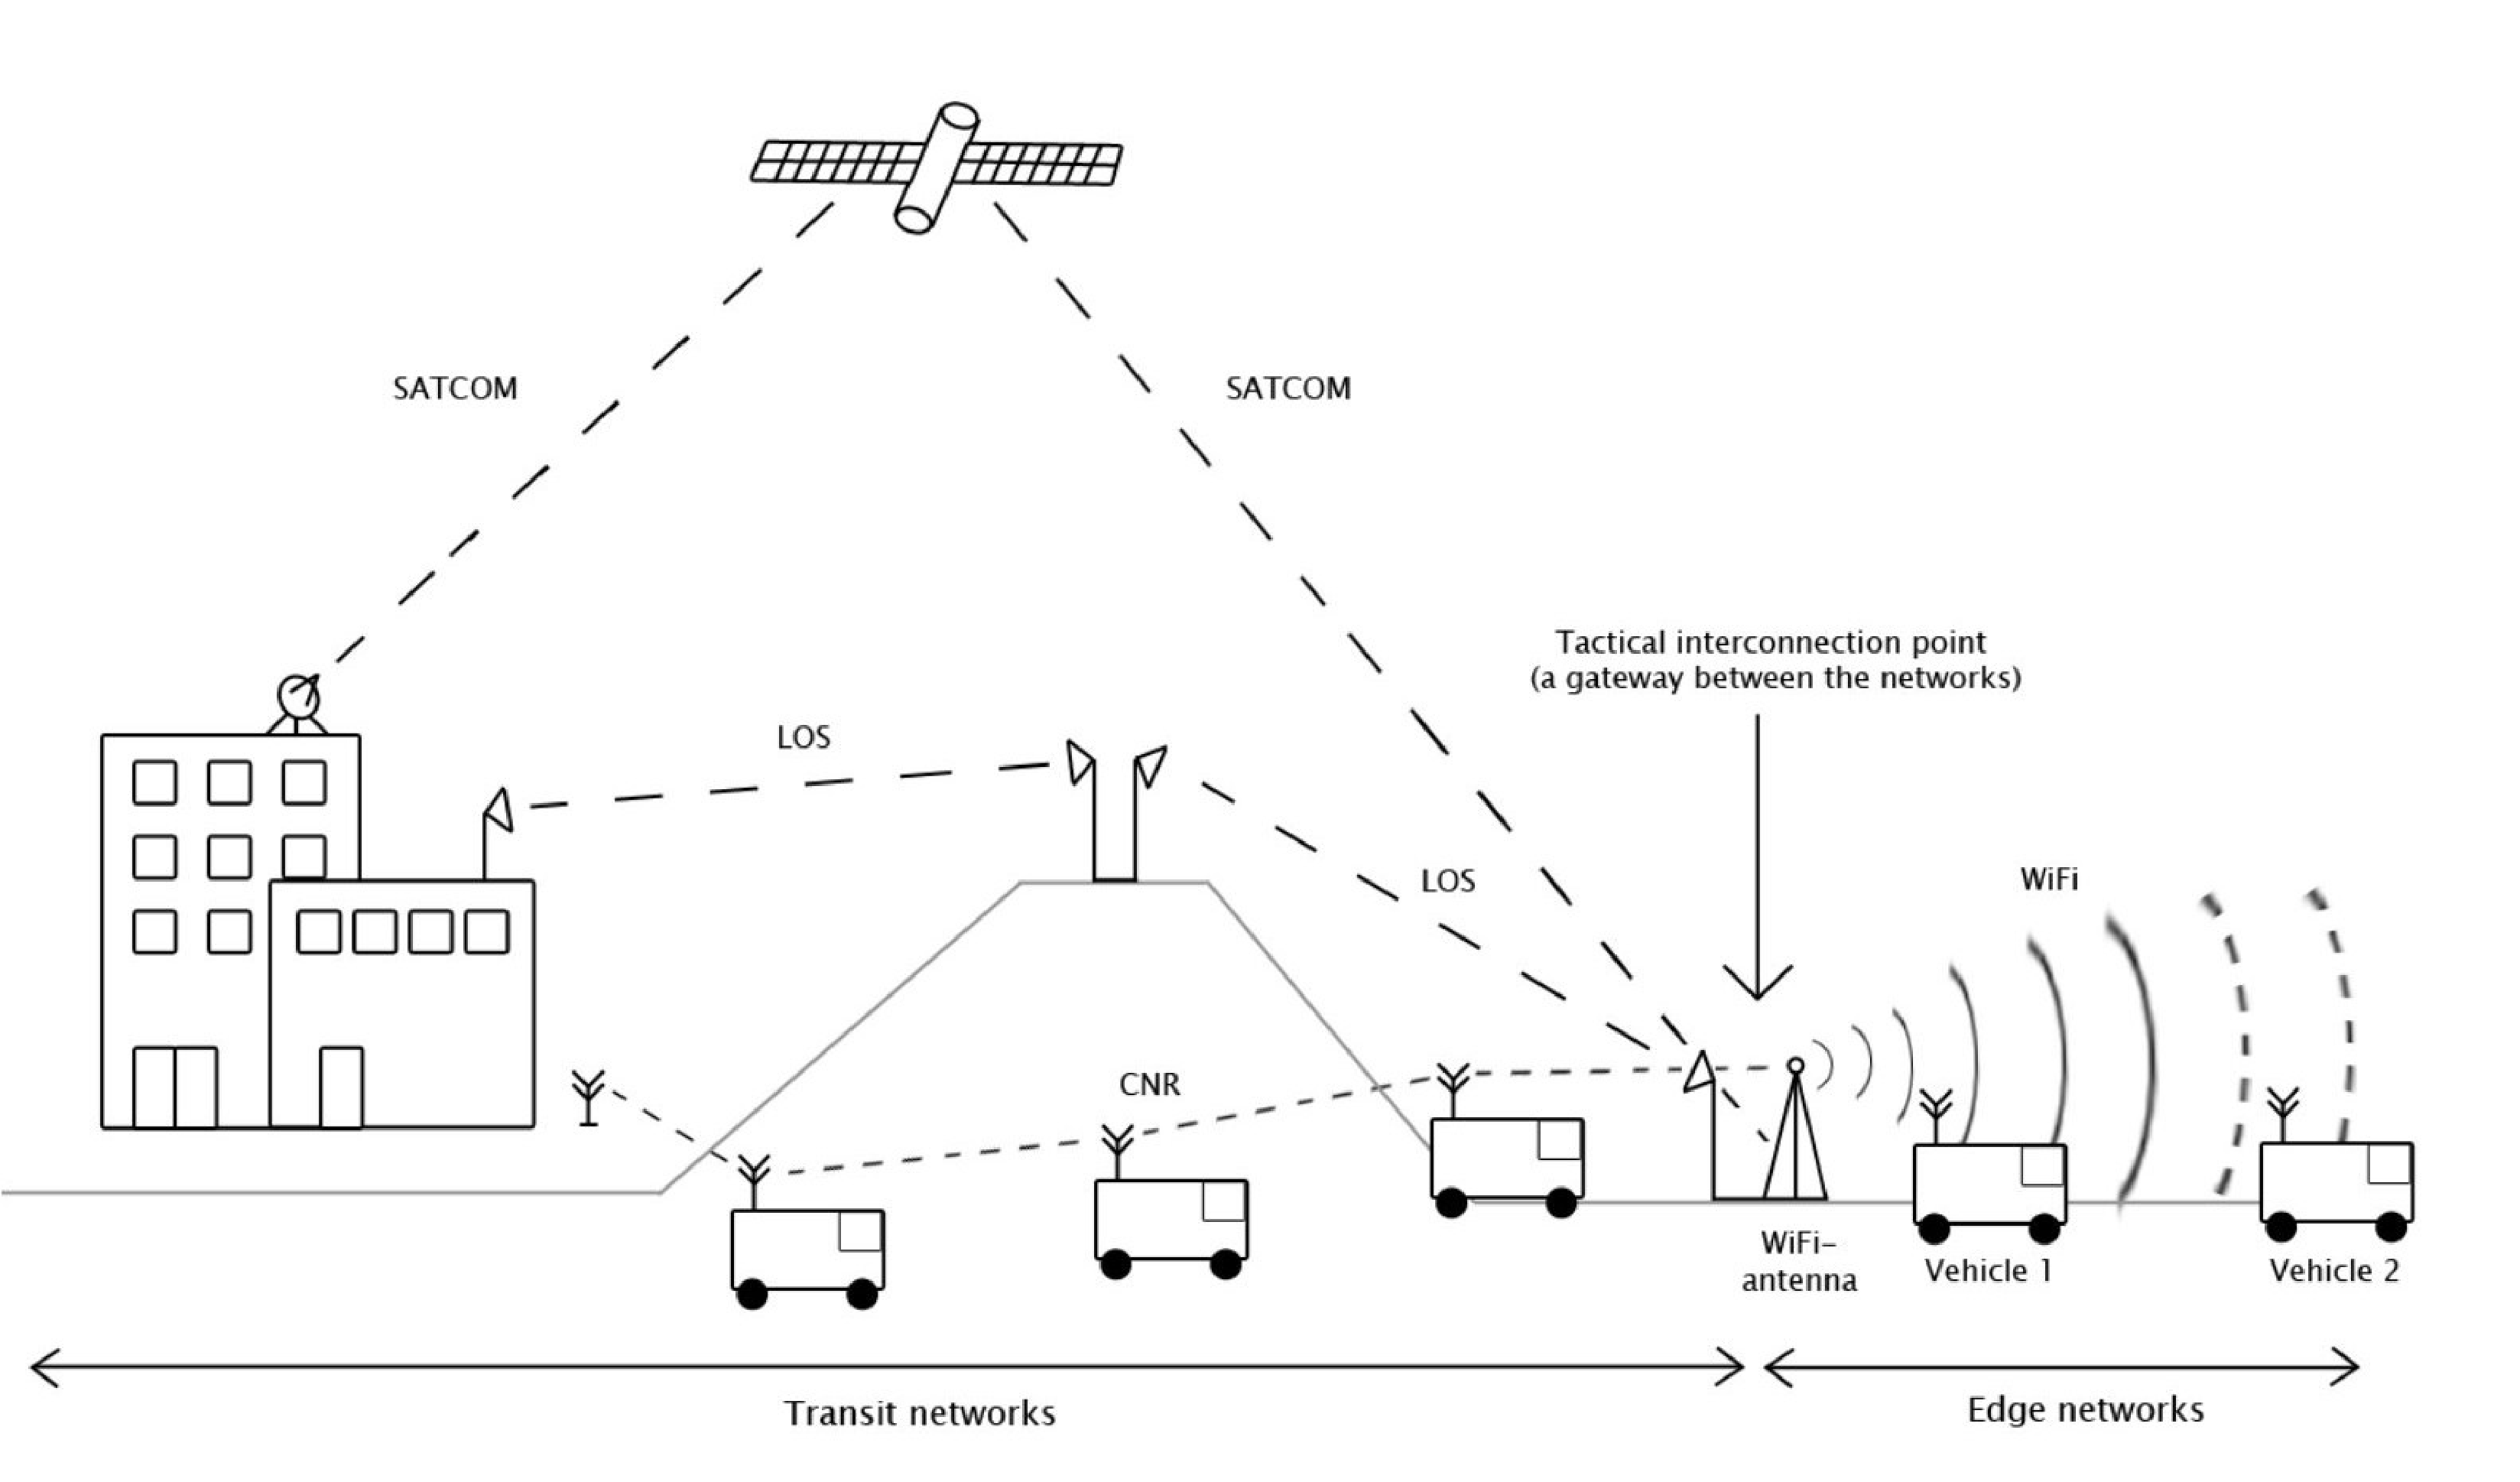
\includegraphics[scale=0.25]{images/networks_overview.pdf}
\caption{Overview of tested networks}
\label{figure-networks-overview}
\end{figure}

In the following sections the test cases is ran for each network
configuration.


\subsection{Satellite communication}

In this test scenario we emulate \gls{satcom}. Low data rate, high delay.
Delay ~ 1100 ms.
Iperf bandwidth:
[  4]   0.00-10.00  sec   491 KBytes   402 Kbits/sec    1             sender
[  4]   0.00-10.00  sec   355 KBytes   291 Kbits/sec                  receiver


\paragraph{Results and analysis}

\begin{table}[h!]
\begin{tabular}{| l | l | l |}
\hline
  \textbf{Test} & \textbf{Transfer time} & \textbf{With compression}\\ \hline
  Without proxy & 14651 ms & N/A ms \\ \hline
  Proxy with HTTP & 13771 ms & 13849 ms \\ \hline
  Proxy with AMQP & 105713 ms & 103230 ms \\ \hline
  Proxy with CoAP & 13720 ms & 13687 ms \\ \hline
\end{tabular}
\caption{RESTful Web service results}
\end{table}

\begin{table}[h!]
\begin{tabular}{| l | l | l |}
\hline
  \textbf{Test} & \textbf{Transfer time} & \textbf{With compression}\\ \hline
  Without proxy & 5680 ms & N/A ms \\ \hline
  Proxy with HTTP & 13771 ms & 3621 ms \\ \hline
  Proxy with AMQP & 23697 ms & 24123 ms \\ \hline
  Proxy with CoAP & 111651 ms & 13687 ms \\ \hline
\end{tabular}
\caption{W3C Web service results}
\end{table}

\subsection{Line-of-Sight}

In this test scenario we emulate so-called \gls{los} networks, which are
characterized by being a radio-based type of network with no physical obstacles
between the nodes in the network. High data rate, low delay and zero error.

Delay ~ 11 ms.
Iperf bandwidth:
[ ID] Interval           Transfer     Bandwidth       Retr
[  4]   0.00-10.00  sec  2.79 MBytes  2.34 Mbits/sec    0             sender
[  4]   0.00-10.00  sec  2.56 MBytes  2.15 Mbits/sec                  receiver



\subsection{WiFi 1}

Placeholder.


\subsection{WiFi 2}

Placeholder

\subsection{Combat Net Radio with Forward Error Correction}

\begin{table}[h!]
\begin{tabular}{| l | l | l |}
\hline
  \textbf{Test} & \textbf{Transfer time} & \textbf{With compression}\\ \hline
  Without proxy & 6235 ms & N/A ms \\ \hline
  Proxy with HTTP & X ms & 3504 ms \\ \hline
  Proxy with AMQP & X ms & 24414 ms \\ \hline
  Proxy with CoAP & X ms & 11210 ms \\ \hline
\end{tabular}
\caption{RESTful Web service results}
\end{table}

\section{Summary}

In this section the results from the tests are presented. These results lead up
to the discussion and conclusion in the next chapter.
